%package list
\documentclass{article}
\usepackage[top=3cm, bottom=3cm, outer=3cm, inner=3cm]{geometry}
\usepackage{multicol}
\usepackage{graphicx}
\usepackage{url}
%\usepackage{cite}
\usepackage{hyperref}
\usepackage{array}
%\usepackage{multicol}
\newcolumntype{x}[1]{>{\centering\arraybackslash\hspace{0pt}}p{#1}}
\usepackage{natbib}
\usepackage{pdfpages}
\usepackage{multirow}
\usepackage[normalem]{ulem}
\useunder{\uline}{\ul}{}
\usepackage{svg}
\usepackage{xcolor}
\usepackage{listings}

\lstdefinestyle{ascii-tree}{
    literate={├}{|}1 {─}{--}1 {└}{+}1 
  }
\lstset{basicstyle=\ttfamily,
  showstringspaces=false,
  commentstyle=\color{red},
  keywordstyle=\color{blue}
}
%\usepackage{booktabs}
\usepackage{caption}
\usepackage{subcaption}
\usepackage{float}
\usepackage{array}

\newcolumntype{M}[1]{>{\centering\arraybackslash}m{#1}}
\newcolumntype{N}{@{}m{0pt}@{}}


%%%%%%%%%%%%%%%%%%%%%%%%%%%%%%%%%%%%%%%%%%%%%%%%%%%%%%%%%%%%%%%%%%%%%%%%%%%%
%%%%%%%%%%%%%%%%%%%%%%%%%%%%%%%%%%%%%%%%%%%%%%%%%%%%%%%%%%%%%%%%%%%%%%%%%%%%
\newcommand{\itemEmail}{aphoccot@unsa.edu.pe}
\newcommand{\itemStudent}{Alejandro Josue Phocco Tapia}
\newcommand{\itemCourse}{Programación Web 2}
\newcommand{\itemCourseCode}{20220589}
\newcommand{\itemSemester}{III}
\newcommand{\itemUniversity}{Universidad Nacional de San Agustín de Arequipa}
\newcommand{\itemFaculty}{Facultad de Ingeniería de Producción y Servicios}
\newcommand{\itemDepartment}{Departamento Académico de Ingeniería de Sistemas e Informática}
\newcommand{\itemSchool}{Escuela Profesional de Ingeniería de Sistemas}
\newcommand{\itemAcademic}{2023 - A}
\newcommand{\itemInput}{Del 29 de Junio 2023}
\newcommand{\itemOutput}{Al 14 Julio 2023}
\newcommand{\itemPracticeNumber}{07}
\newcommand{\itemTheme}{Python - Django}
%%%%%%%%%%%%%%%%%%%%%%%%%%%%%%%%%%%%%%%%%%%%%%%%%%%%%%%%%%%%%%%%%%%%%%%%%%%%
%%%%%%%%%%%%%%%%%%%%%%%%%%%%%%%%%%%%%%%%%%%%%%%%%%%%%%%%%%%%%%%%%%%%%%%%%%%%

\usepackage[english,spanish]{babel}
\usepackage[utf8]{inputenc}
\AtBeginDocument{\selectlanguage{spanish}}
\renewcommand{\figurename}{Figura}
\renewcommand{\refname}{Referencias}
\renewcommand{\tablename}{Tabla} %esto no funciona cuando se usa babel
\AtBeginDocument{%
	\renewcommand\tablename{Tabla}
}

\usepackage{fancyhdr}
\pagestyle{fancy}
\fancyhf{}
\setlength{\headheight}{30pt}
\renewcommand{\headrulewidth}{1pt}
\renewcommand{\footrulewidth}{1pt}
\fancyhead[L]{\raisebox{-0.2\height}{
\includegraphics[width=3cm]{img/logo_episunsa.png}}}
\fancyhead[C]{\fontsize{7}{7}\selectfont	\itemUniversity \\ \itemFaculty \\ \itemDepartment \\ \itemSchool \\ \textbf{\itemCourse}}
\fancyhead[R]{\raisebox{-0.2\height}{
\includegraphics[width=1.2cm]{img/logo_abet}}}
\fancyfoot[L]{Estudiante Alejandro Phocco Tapia}
\fancyfoot[C]{\itemCourse}
\fancyfoot[R]{Página \thepage}

% para el codigo fuente
\usepackage{listings}
\usepackage{color, colortbl}
\definecolor{dkgreen}{rgb}{0,0.6,0}
\definecolor{gray}{rgb}{0.5,0.5,0.5}
\definecolor{mauve}{rgb}{0.58,0,0.82}
\definecolor{codebackground}{rgb}{0.95, 0.95, 0.92}
\definecolor{tablebackground}{rgb}{0.8, 0, 0}

\lstset{frame=tb,
	language=bash,
	aboveskip=3mm,
	belowskip=3mm,
	showstringspaces=false,
	columns=flexible,
	basicstyle={\small\ttfamily},
	numbers=none,
	numberstyle=\tiny\color{gray},
	keywordstyle=\color{blue},
	commentstyle=\color{dkgreen},
	stringstyle=\color{mauve},
	breaklines=true,
	breakatwhitespace=true,
	tabsize=3,
	backgroundcolor= \color{codebackground},
}

\begin{document}
	\vspace*{10px}
	
	\begin{center}	
		\fontsize{17}{17} \textbf{ Informe de Laboratorio \itemPracticeNumber}
	\end{center}
	\centerline{\textbf{\Large Tema: \itemTheme}}
	%\vspace*{0.5cm}	

	\begin{flushright}
		\begin{tabular}{|M{2.5cm}|N|}
			\hline 
			\rowcolor{tablebackground}
			\color{white} \textbf{Nota}  \\
			\hline 
			     \\[30pt]
			\hline 			
		\end{tabular}
	\end{flushright}	

	\begin{table}[H]
		\begin{tabular}{|x{4.7cm}|x{4.8cm}|x{4.8cm}|}
			\hline 
			\rowcolor{tablebackground}
			\color{white} \textbf{Estudiante} & \color{white}\textbf{Escuela}  & \color{white}\textbf{Asignatura}   \\
			\hline 
			{\itemStudent \par \itemEmail} & \itemSchool & {\itemCourse \par Semestre: \itemSemester \par Código: \itemCourseCode}     \\
			\hline 			
		\end{tabular}
	\end{table}		
	
	\begin{table}[H]
		\begin{tabular}{|x{4.7cm}|x{4.8cm}|x{4.8cm}|}
			\hline 
			\rowcolor{tablebackground}
			\color{white}\textbf{Laboratorio} & \color{white}\textbf{Tema}  & \color{white}\textbf{Duración}   \\
			\hline 
			\itemPracticeNumber & \itemTheme & 04 horas   \\
			\hline 
		\end{tabular}
	\end{table}
	
	\begin{table}[H]
		\begin{tabular}{|x{4.7cm}|x{4.8cm}|x{4.8cm}|}
			\hline 
			\rowcolor{tablebackground}
			\color{white}\textbf{Semestre académico} & \color{white}\textbf{Fecha de inicio}  & \color{white}\textbf{Fecha de entrega}   \\
			\hline 
			\itemAcademic & \itemInput &  \itemOutput  \\
			\hline 
		\end{tabular}
	\end{table}
	
	\section{Tarea}
	\begin{itemize}		
		\item Recreacion de los videos proporcionados en el aula virtual sobre relaciones one to many y many to many, asi como la generacion de pdf's y el envio de emails.
	\end{itemize}
        \begin{figure}[H]
		\centering
		
\includegraphics[width=0.25\textwidth,keepaspectratio]{img/django.png}
	\end{figure}

	\section{URL de Repositorio Github}
	\begin{itemize}
		\item URL para el laboratorio 07 en el Repositorio GitHub.
		\item \url{https://github.com/AlejandroPhoccoTapia/Lab07-PW2-AlejandroPhocco}
	\end{itemize}
	
	\section{Ejercicios}  
 
	\subsection{Relaciones One to Many}
        Veremos los modelos que permiten la relacion de uno a muchos.

        \begin{lstlisting}[language=bash,caption={models.py de la app}][H]
         from django.db import models
        
        # Create your models here.
        
        class Author(models.Model):
            name = models.CharField(max_length=10)
        
            def __str__(self):
                return self.name
        
        class Book(models.Model):
            name = models.CharField(max_length=10)
            author = models.ForeignKey(Author, on_delete=models.CASCADE)
        
            def __str__(self):
                return self.name
	\end{lstlisting}
        Aqui la relacion se da mediante  el campo ForeignKey.

        \subsection{Relaciones Many to Many}
        Veremos los modelos que permiten la relacion de uno a muchos.

        \begin{lstlisting}[language=bash,caption={models.py de la app}][H]
         from django.db import models
        
        # Create your models here.
        
        class Class(models.Model):
            name = models.CharField(max_length=10)
        
            def __str__(self):
                return self.name
            
        class Student(models.Model):
            name = models.CharField(max_length=10)
            nameClass =  models.ManyToManyField(Class)
        
            def __str__(self):
                return self.name
	\end{lstlisting}
        Aqui la relacion se da mediante  el campo ManyToManyField.
        
        \subsection{Generaciónn de pdf}
        
        \begin{itemize}
            \item Analizando las url de la app
        \end{itemize}
        \begin{lstlisting}[language=bash,caption={Archivo urls.py}][H]
            from django.urls import path
            from . import views
            
            urlpatterns = [
              path('pdf/', views.GeneratePDF.as_view(), name='PDF'),
            ]
	\end{lstlisting}
        Como vemos tendremos una url "pdf" que sera la que imprima un pdf como tal haciendo uso de una view; esto teniendo en cuenta que importaremos las urls de la aplicacion pdf.

        \begin{itemize}
            \item En la app pdf, analizaremos el archivo utils.py
        \end{itemize}
        \begin{lstlisting}[language=bash,caption={Archivo pdf/utils.py}][H]
            from io import BytesIO
            from django.http import HttpResponse
            from django.template.loader import get_template
            
            from xhtml2pdf import pisa
            
            def render_to_pdf(template_src, context_dict={}):
                template = get_template(template_src)
                html  = template.render(context_dict)
                result = BytesIO()
                pdf = pisa.pisaDocument(BytesIO(html.encode("ISO-8859-1")), result)
                if not pdf.err:
                    return HttpResponse(result.getvalue(), content_type='application/pdf')
                return None
	\end{lstlisting}
        En esta función toma una plantilla HTML, la renderiza con los datos del contexto y la convierte en un archivo PDF utilizando xhtml2pdf. Luego, devuelve una respuesta HTTP que contiene el PDF generado. \newline

         \begin{itemize}
            \item Vistas de la app
        \end{itemize}
        \begin{lstlisting}[language=bash,caption={Archivo pdf/views.py}][H]
            from django.shortcuts import render

            from django.http import HttpResponse
            from django.template.loader import get_template
            from django.views.generic import View
            
            from .utils import render_to_pdf #created in step 4
            
            class GeneratePdf(View):
                def get(self, request, *args, **kwargs):
                    template = get_template('invoice.html')
                    context = {
                         'today': "Today", 
                         'amount': 1339.99,
                        'customer_name': 'Cooper Mann',
                        'invoice_id': 1233434,
                    }
                    html = template.render(context)
                    pdf = render_to_pdf('invoice.html',context)
                    if pdf:
                        response = HttpResponse(pdf, content_type='application/pdf')
                        filename = "Invoice_%s.pdf"%("12341231")
                        content = "inline; filename='%s'"%(filename)
                        download = request.GET.get("download")
                        if download:
                            content = "attachment; filename='%s'" %(filename)
                        response['Content-Disposition']=content
                        return response  
            
                    return HttpResponse("Not Found")
	\end{lstlisting}
        Esta vista basada en clase permite generar y devolver un archivo PDF a partir de una plantilla HTML cuando se realiza una solicitud HTTP GET a la vista. El archivo PDF puede ser descargado o mostrado en el navegador según los parámetros proporcionados en la URL de la solicitud. A resaltar que se importa la función render\_to\_pdf desde un archivo utils.py, que se supone que contiene una función personalizada para generar un archivo PDF a partir de una plantilla HTML.\newline

         \begin{itemize}
            \item HTML de la app
        \end{itemize}
        \begin{lstlisting}[language=bash,caption={Archivo TemplateToPDF/templates/pdf.html}][H]
            <!DOCTYPE html>
            <html lang="en">
            <head>
              <meta charset="UTF-8">
              <meta name="viewport" content="width=device-width, initial-scale=1.0">
              <title>Enviar</title>
            </head>
            <body>
              <h1>Laboratorio {{lab}}</h1>
              <h2>Hola {{name}}</h2>
            </body>
            </html>
	\end{lstlisting}
        Esta es una plantilla basica que utiliza el numero de laboratorio y el nombre del alumno\newline

        
        \begin{itemize}
            \item Demostracion en navegador\newline
            
        \end{itemize}
        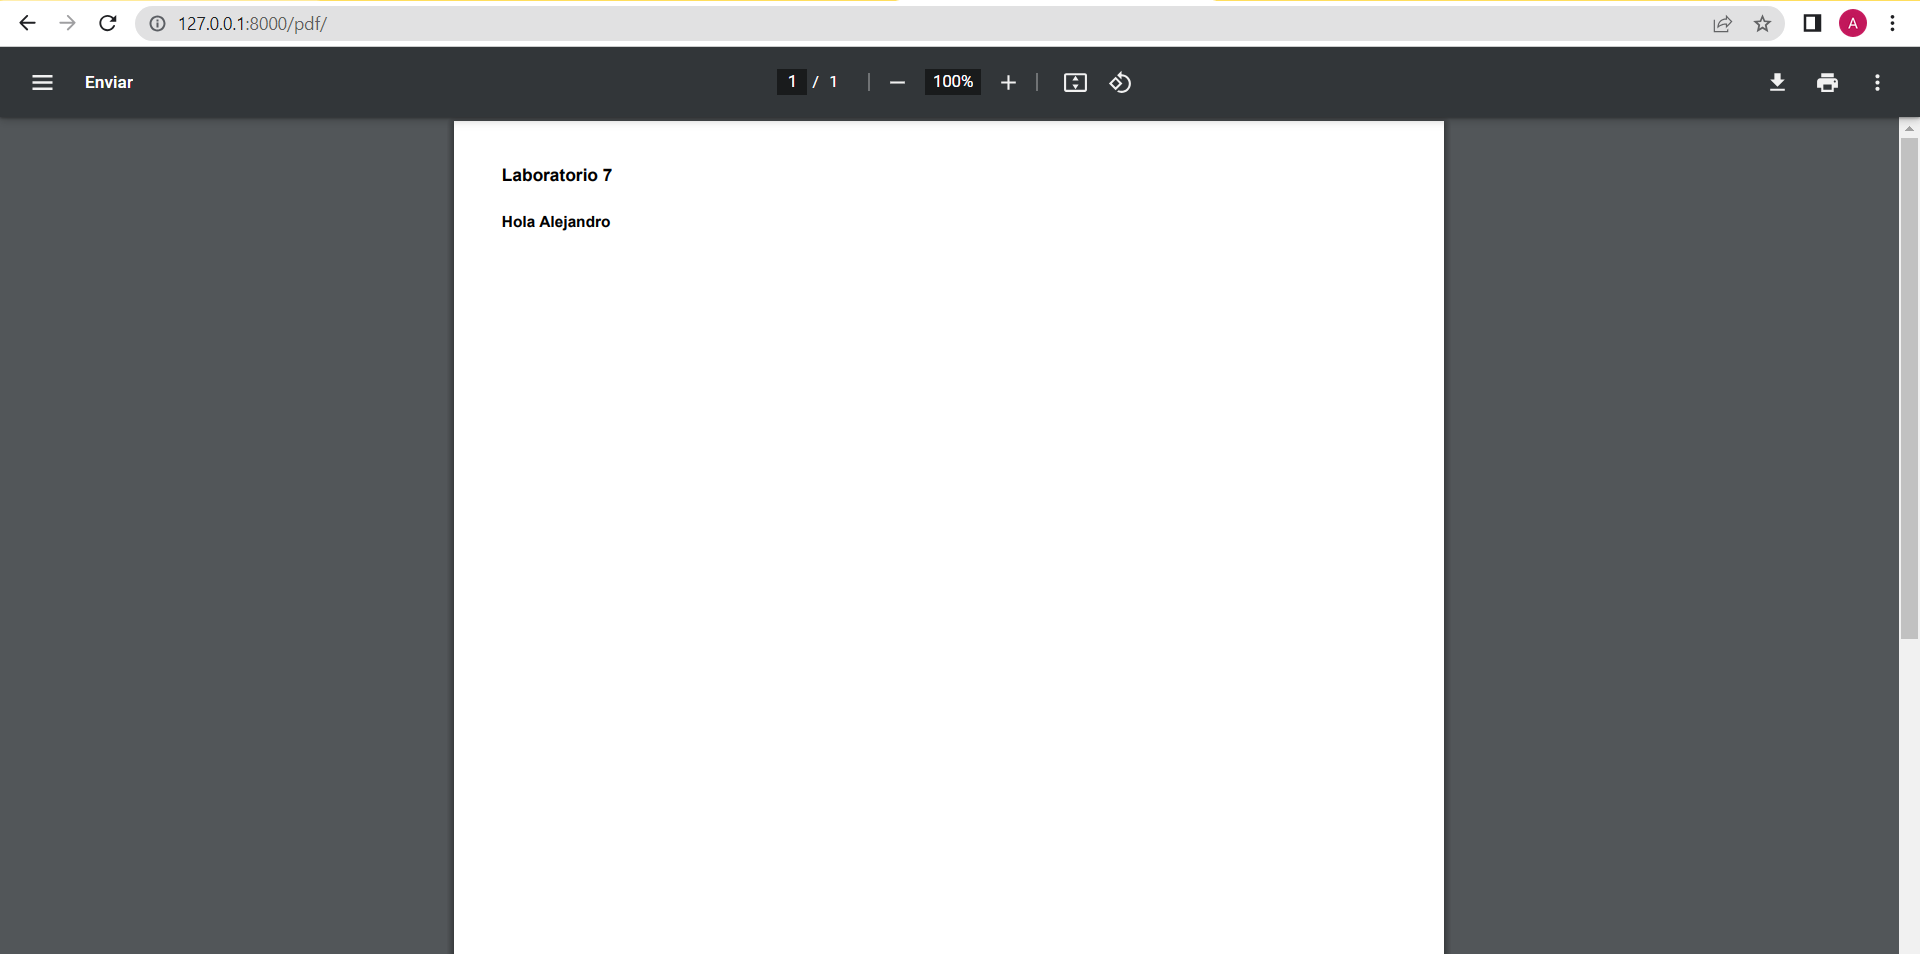
\includegraphics[width=16cm]{img/PDF DEMOSTRACION IMG.png}
        \newline Observamos que el pdf se creo efectivamente con los datos enviados como contexto.
        
        \subsection{Envio de email}
        
        \begin{itemize}
            \item Analizando la configuracion del proyecto para enviar emails
        \end{itemize}
        \begin{lstlisting}[language=bash,caption={Archivo settings.py}][H]
            EMAIL_HOST = 'smtp.gmail.com' #Estoy usando el servicio de gmail
            EMAIL_PORT = 587
            EMAIL_HOST_USER = 'aphoccot@unsa.edu.pe' #Uso de mi correo institucional
            EMAIL_HOST_PASSWORD = 'qilregazjfiwoebh'
            EMAIL_USE_TLS = True
            EMAIL_USE_SSL = False
	\end{lstlisting}
        Aqui configuraremos el servicio de mensajeria que utilizaremos, el puerto que utiliza y la cuenta que usara para enviar los correos.
        \newline
        
         \begin{itemize}
            \item En la app SendingEmails, analizaremos el archivo urls.py
        \end{itemize}
        \begin{lstlisting}[language=bash,caption={Archivo SendingEmails/urls.py}][H]
            from django.urls import path, include
            from . import views
            
            urlpatterns = [
              path('email/',  views.send),
            ]

	\end{lstlisting}
        Crea una ruta email y llama a la funcion send de su vista que se encargara de enivar el mail.\newline

        \begin{itemize}
            \item Analizaremos el archivo views.py
        \end{itemize}
        \begin{lstlisting}[language=bash,caption={Archivo SendingEmails/views.py}][H]
            from django.shortcuts import render
            from django.core.mail import send_mail
            
            def send(request):
                send_mail('EMAIL PRUEBA DJANGO',
                          'Sirve :V',
                          'aphoccot@unsa.edu.pe',
                          ['pocochuk12345@gmail.com'],
                          fail_silently=False)
                return render(request, 'email.html')
	\end{lstlisting}
         Esta vista en Django utiliza la función send\_mail y luego retorna la plantilla emal.html\newline

         \begin{itemize}
            \item Analizaremos el archivo templates/email.html
        \end{itemize}
        \begin{lstlisting}[language=bash,caption={Archivo SendingEmails/templates/email.html}][H]
            <!DOCTYPE html>
            <html lang="en">
            <head>
              <meta charset="UTF-8">
              <meta name="viewport" content="width=device-width, initial-scale=1.0">
              <title>Envio de Email</title>
            </head>
            <body>
              Se envio el email con exito
            </body>
            </html>
	\end{lstlisting}
         Esta es una plantilla simple que contiene un mensaje que confirma que el correo ha sido enviado.\newline

        \begin{itemize}
            \item Demostracion en navegador\newline
            
        \end{itemize}
        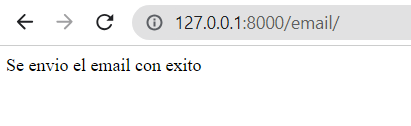
\includegraphics[width=16cm]{img/correoEnviado.png}
        \newline Vemos que la pagina nos confirma que el correo ha sido enviado.

        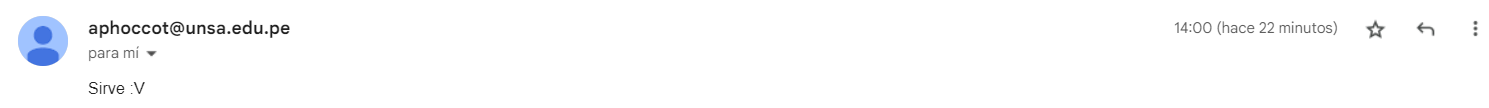
\includegraphics[width=16cm]{img/correo recibido.png}
        \newline Comprobamos que efectivamente llego correo, con el contenido que le especificamos.
        \newline
        \newline\newline 
        Link donde esta alojado el video (FlipGrid):\newline
        GRUPO:
        \url{https://flip.com/groups/14644257/topics/37115679/responses/430314063}
        
\section{Cuestionario}
	- Sin cuestionario -	
 \newpage
 \section{Conclusiones}
	\begin{itemize}
		\item Django es un excelente framework que nos facilita la creacion de tablas con relacion de uno a muchos o de muchos a muchos.
            \item Djando ofrece una gran facilidad para crear pdfs y para enviar email personalizados, de una forma sencilla, efectiva y comoda.
	\end{itemize}	
\clearpage

\section{Referencias}
\begin{itemize}	
    \item \url{https://www.w3schools.com/python/python_reference.asp}
    \item \url{https://docs.djangoproject.com/en/4.2/topics/email/}
    \item \url{https://www.scaler.com/topics/django/relationships-in-django-models/}
    \item \url{https://docs.djangoproject.com/en/4.2/howto/outputting-pdf/}
\end{itemize}	
	
%\clearpage
%\bibliographystyle{apalike}
%\bibliographystyle{IEEEtranN}
%\bibliography{bibliography}
			
\end{document}